\chapter{Microservices}
\label{chap:Microservices}
Ein Microservices-System besteht aus vielen verteilten Anwendungen (Dienste), welche man selber ebenfalls Microservices nennt. Dabei wird versucht, eine komplexe Anwendungen, in einzelne Dienste aufzuteilen.

\begin{quotation}
    \frqq Modularisierung ist nichts Neues. Schon lange werden große Systeme in kleine Module unterteilt, um Software einfacher zu erstellen, zu verstehen und weiterzuentwickeln. Das Neue: Microservices nutzen als Module einzelne Programme, die als eigene Prozesse laufen. Der Ansatz basiert auf der UNIX-Philosophie. Sie lässt sich auf drei Aspekte reduzieren:\flqq\cite[S. 2]{EWolff2016:Microservices}
\end{quotation}

\begin{itemize}
    \item Ein Programm soll nur eine Aufgabe erledigen, und das soll es gut machen.
    \item Programme sollen zusammenarbeiten können.
    \item Nutze eine universelle Schnittstelle. In UNIX sind das beispielsweise Textströme.
\end{itemize}
Diese Art der Aufteilung wurde schon lange von großen Unternehmen wie Amazon oder Google genutzt, jedoch fehlte lange Zeit ein Begriff für dieses Paradigma.
\\\\
Der Begriff Microservices ist nicht eindeutig definiert. Als erste Näherung dienen, nach Eberhard Wolff \cite[S. 2]{EWolff2016:Microservices}, folgende Kriterien:

\begin{itemize}
    \item Microservices ist ein Modularisierungskonzept. Sie dienen dazu, ein großes Software-System aufzuteilen - und beeinflussen die Organisation und die Software-Entwicklungsprozesse.
    \item Microservices können unabhängig von Änderungen an anderen Microservices in Produktion gebracht werden.
    \item Microservices können in unterschiedlichen Technologien implementiert sein. Es gibt keine Einschränkung auf eine bestimmte Programmiersprache oder Plattform.
    \item Microservices haben einen eigenen Datenhaushalt: eine eigene Datenbank - oder ein vollständig getrenntes Schema in einer gemeinsamen Datenbank.
    \item Microservices können eigene Unterstützungsdienste mitbringen, beispielsweise eine Suchmaschine oder eine spezielle Datenbank. Natürlich gibt es eine gemeinsame Basis für alle Microservices - beispielsweise die Ausführung virtueller Maschinen.
    \item Microservices sind eigenständige Prozesse - oder virtuelle Maschinen, um auch die Unterstützungsdienste mitzubringen.
    \item Dementsprechend müssen Microservices über das Netzwerk kommunizieren. Dazu nutzen Microservices Protokolle, die lose Kopplung unterstützen. Das kann beispielsweise RE
    ST sein - oder Messaging-Lösungen.
\end{itemize}

Grundsätzlich kann man Microservices in drei Kategorien einteilen:
\begin{description}
    \item[Producer] Ein Service der etwas produziert oder auf eine Anfrage reagiert. Das reicht von Daten aus einer Datenbank zu extrahieren bis hin zu komplexen Berechnungen.
    \item[Consumer] Ein Service oder eine Anwendung, welche einen oder mehrere produzierende Services verwendet und entweder weiterverarbeitet oder ausgibt. Im Falle der Weiterverarbeitung ist ein Consumer ebenfalls ein Producer.
    \item[Self-Contained System (SCS)] \frqq "`Microservice mit UI"' oder "'Self-Contained System"' wie es Stefan Tilkov nennt, sind in sich abgeschlossene Systeme. [..] Sie enthalten eine UI und sollten möglichst nicht mit anderen SCS kommunizieren.\flqq \cite[vgl S. 55]{EWolff2016:Microservices}.
\end{description}

\section{Aufbau von Microservices}
\label{sec:Aufbau}
Wie bereits erwähnt, sind Microservices eigenständige Dienste. Sie müssen so gebaut sein, dass sie möglichst ohne Abhängigkeiten funktionieren. Um das zu realisieren dürfen Microservices nur lose gekoppelt sein. Damit ist gemeint, dass der Dienst seine Aufgabe selbständig erledigen kann ohne weiter Dienste in Anspruch zu nehmen. Bei "`Self-Contained Systems"' ist ebenfalls ist ebenfalls eine UI vorhanden. Damit ist das System für sich selbständig und stellt ebenfalls alle nötigen Eigenschaften bereit für die Darstellung von Informationen. Müssen jedoch andere Dienste verwendet werden, sollte darauf geachtet werden, dass diese austauschbar bleiben und nicht fest mit miteinander verbunden sind. Ist ein Dienst fest mit einem anderen verbunden, sollte die Notwendigkeit des Dienstes infrage gestellt werden.
\\\\
In direkter Konkurrenz stehen konsumierende Dienste, welche produzierende Dienste verwenden müssen, um die eigenen Aufgaben fertig zu stellen. Konsumierende Dienste werden jedoch häufig als Middleware verwendet, um mehrere Daten aufzubereiten. Ein Konsumierender Dienst könnte zum Beispiel die Aufgabe haben eine Webseite darzustellen oder Informationen zu aggregieren.
\\\\
Damit ein Dienst selbständig bleibt, besitzt dieser alle dafür notwendigen Ressourcen. Hierzu zählt, unter anderem, eine eigene Datenbank. Dadurch kann das Schema der Datenbank frei verändert werden, ohne, dass weitere Teile des Systems beeinflusst werden. Es ist jedoch darauf zu achten, dass die Schnittstelle des Dienstes, worüber dieser von anderen Diensten ansprechbar ist, nicht grundlegend verändert wird.
\\\\
Geht man von \textit{Self-Contained Systems} aus, besitzen Microservices zusätzlich noch eigene UI-Elemente. Dadurch ist nur noch ein aggregierender Dienst notwendig, welcher alle Informationen zusammenfasst.

\begin{figure}[htb]
	\centering 
	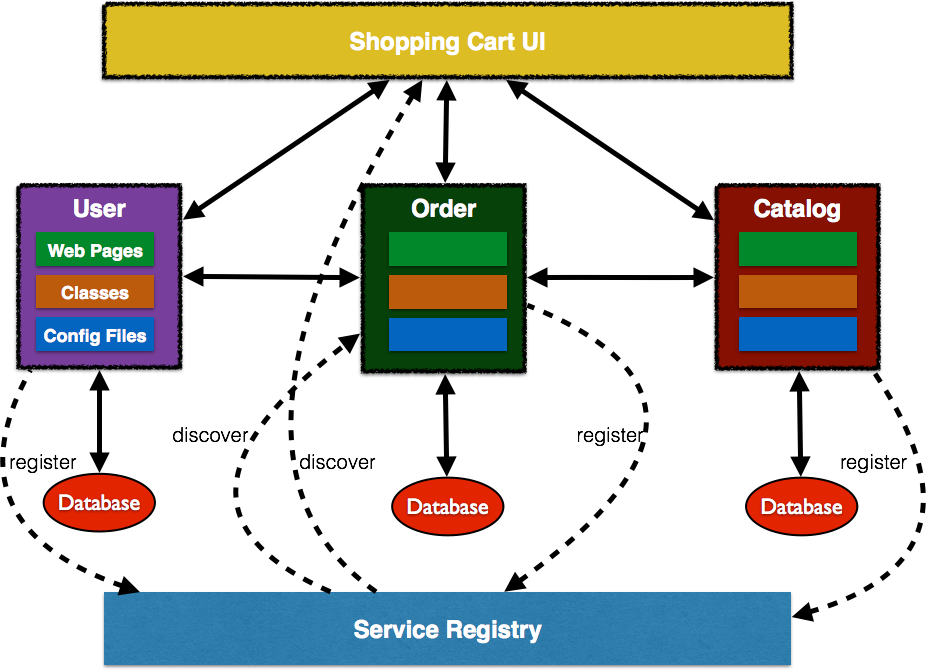
\includegraphics[width=\linewidth]{content/images/javaee-microservices}\
	\quelle\url{http://blog.arungupta.me/monolithic-microservices-refactoring-javaee-applications/}
	\caption{Microservice Architektur\\}
	\label{fig:MicroserviceArchitektur} 
\end{figure}

\section{Gr"o\ss e von Microservices}
\label{sec:groesseMicroservice}
\begin{quotation}
    \frqq Der Name "`Microservices"' verrät schon, dass es um die Servicegröße geht - offensichtlich sollen die Services klein sein."\cite[S. 31]{EWolff2016:Microservices} Es gibt verschiedene Möglichkeiten die Größe von Programmen zu ermitteln. Eine Variante ist zum Beispiel das Zählen von  Lines of Code (LOC), jedoch hat diese Methode auch Nachteile. Denn die Anzahl der Codezeilen hängen stark von der verwendeten Programmiersprache ab. Einige Programmiersprachen benötigen mehr Zeilen Code, um eine bestimmte Tätigkeit abzubilden, als andere.
    \\
    Die Größe von Services sollte jedoch nicht von zentraler Bedeutung sein, denn eine untere Grenze gibt es für Services nicht. "Wohl aber eine obere Grenze: Wenn der Microservice so groß ist, dass er von einem Team nicht mehr weiterentwickelt werden kann, ist sie zu groß. Ein Team sollte dabei eine Größe haben, wie sie für agile Prozesse besonders gut funktioniert. Das sind typischerweise drei bis neun Personen.\flqq\cite[S. 34]{EWolff2016:Microservices}
\end{quotation}

Bei der Größe eines Services ist darauf zu achten, das ein Service nicht zu viele oder zu wenige Funktionen besitzt. Wie bereits beschrieben, sind Microservices modulare, lose gekoppelte Services. Wird ein Service zu klein angesetzt, können daraus Abhängigkeiten zu anderen Services entstehen und damit das Gesetzt der losen Kopplung verletzten. Besitzt hingegen ein Service zu viele Funktionen, wird es meistens nicht mehr als Microservice angesehen, da es nicht eine, sondern mehrere Aufgaben übernimmt und diese wahrscheinlich nicht mehr gut erledigen kann.

\section{Orchestration vs Choreographie}
\label{sec:orchestrationvschoreographie}
Möchte man ein Microservice System aufbauen, stellt sich die Frage, wie einzelne Services strukturiert werden und wie diese untereinander kommunizieren sollen. Ein bestimmter Vorgang startet in der Regel bei einem Service. Nun muss man entscheiden ob weitere Services hinzugezogen, beziehungsweise informiert werden müssen.
Je nach Anwendungsfall muss man sich zwischen Service Orchestration und Choreographie entscheiden. Dabei ist es fast unmöglich ein ganzes Microservice-System aus nur einem der beiden Varianten zu bauen.

% [Seite 66 EWolff2016] Technologische Wahlfreiheit
\subsection{Herausforderung}
\label{sec:Herausforderung}
Der Ausfall eines Services kann im schlechtesten Fall dazu führen, dass alle anderen Microservices nicht mehr funktionieren. Um das zu verhindern muss klar definiert werden, was Microservices in dieser Situation tun sollen. Zusätzlich muss, sofern Datenbankoperationen eine wichtige Rolle spielen, das Problem der einheitlichen Transaktion gelöst werden. Wenn zum Beispiel eine Operation Daten über verschiedene Microservices in Datenbanken schreibt, muss bei nicht Erreichbarkeit oder dem Auftreten eines Fehlers in einem Microservices ein einheitlicher Rollback durchgeführt werden, um keine inkonsistente Dateien im System zu erzeugen.
\\\\
Daneben muss sichergestellt werden, dass Nachrichten erfolgreich verarbeitet werden und auch bei mehrfachen senden einer Nachricht keine Fehler auftreten. Dafür müssen Microservices Idempotent sein. Das Heißt, dass eine Wiederholte Aktion (mit gleichen Daten) nicht zu unterschiedlichen Resultaten führt. Wird keine Idempotenz sichergestellt, kann dies zu unerwarteten und unerwünschten Ereignissen führen.
\\\\
Eine weitere Herausforderung besteht in dem Grundkonzept von Microservices. Da nicht definiert ist, welche Programmiersprache für Microservices verwendet wird, kann ein Service zum Beispiel in Java, ein anderes in Scala oder Python geschrieben werden. Es muss daher dafür gesorgt werden, dass die einzelnen Services untereinander interoperabel sind. Um das zu gewährleisten, müssen die Schnittstellen möglichst einheitlich und auf dem gleichen Protokoll aufbauend programmiert werden. Hier bieten REST-Schnittstellen eine gute Lösung. Diese beruhen auf dem HTTP-Protokoll. Zusätzlich bietet das HTTP-Protokoll die Möglichkeit, ein einheitliches Medium, wie zum Beispiel XML oder JSON, als Informationsträger zu nutzen. Dabei kann theoretisch jeder Microservice mit jedem anderen Microservice kommunizieren, sofern die Schnittstellen einheitlich definiert sind.
\\\\
Damit die Schnittstellen genutzt werden können, müssen die Kommunikationskanäle dafür existieren. Nach dem Gesetz von Conway, bedeutet dies, dass die einzelnen Abteilungen bzw. Teams die nötigen Kanäle schaffen müssen.
\newpage
\begin{figure}[htb]
	\centering 
	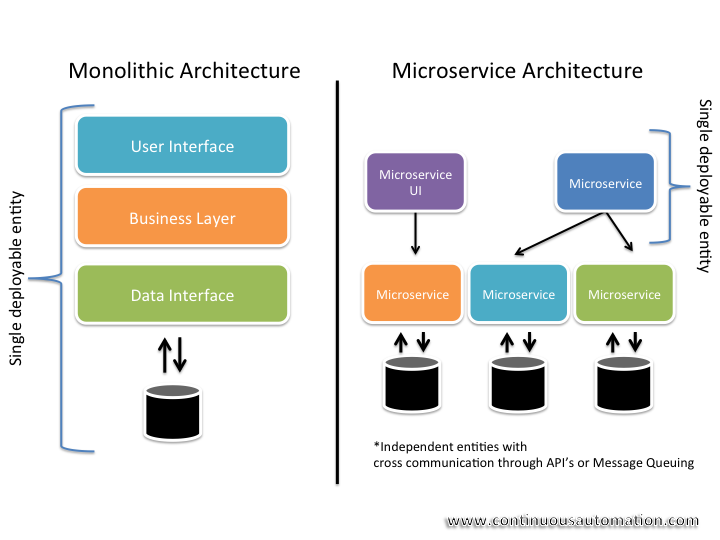
\includegraphics[width=\linewidth]{content/images/570495-slide1}\
	\quelle\url{https://dzone.com/articles/scalable-cloud-computing-with-microservices}
	\caption{Monolithisch vs Microservice Architektur\\}
	\label{fig:MonoVSMicroArchitektur} 
\end{figure}
Im Unterschied zu monolithischen Anwendungen, bei der alles in einer Anwendung ist, sind Microservices einer Fachlichkeit zugeordnet und werden von den jeweiligen Teams entwickelt und verwaltet. Wird eine neue Funktion benötigt, welche nicht in der eigenen Fachlichkeit liegt, muss das entsprechende Team damit beauftragt werden, diese zu implementieren.

\section{PUSH- VS PULL-Architektur}
\label{sec:PushPullArchitektur}
Grundlegend können Microservices mit Hilfe zwei verschiedener Kommunikations-Architekturen kommunizieren, PUSH- und PULL-Architektur. Dabei ist jedoch nicht ausgeschlossen, dass sobald eine Architektur gewählt worden ist, die andere nicht mehr genutzt werden kann. Genauso wie bei der Entscheidung über die Kommunikationsstruktur (siehe \ref{subsec:orchestration} \nameref{subsec:orchestration}), kann es von Vorteil sein, beide Architekturen zu nutzen.
\\\\
\textbf{PULL-Architektur}\\
Eine PULL-Architektur basiert auf einen einfachen Request-Replay-Schema. Dementsprechend ist das Web PULL-basiert.
Der Browser macht eine Anfrage an einen Server, dieser wiederum verarbeitet die Anfrage und liefert eine Antwort (Replay) zurück. Dies hat den Vorteil, dass nicht lange auf eine Antwort gewartet werden muss und sich die teilhabenden Kommunikationspartner gegenseitig kennen. Ein Nachteil jedoch ist es, dass dadurch weitgehend eine synchrone Kommunikation stattfindet und eine Antwort häufig nicht gleichzeitig an mehrere Empfänger senden kann.
\\\\
\textbf{PUSH-Architektur}\\
Eine PUSH-Architektur wird eingesetzt, wenn man verschiedene Kommunikationspartner über bestimmte Ereignisse informieren möchte oder eine Rückantwort ist nicht erforderlich. Zum Beispiel muss eine Registrierung in unserem fiktiven Unternehmen möglich sein. Dabei sendet der Microservice der für die Registrierung zuständig ist eine einfache Event-Nachricht, wie Benutzer XY hat sich Registriert. Im Hintergrund erhalten anderer Microservices diese Nachricht und führen zusätzliche Aktionen durch, wie das erstellen des Warenkorbs oder das anlegen des Profils.
\\\\
Bei der PUSH-Architektur stehen meist nicht die Kommunikationspartner, sondern die Informationen im Vordergrund. Dafür wird meistens ein eigenständiger Service (Broadcaster) eingesetzt, der die Verteilung dieser Informationen übernimmt. Dabei kann ein Service als Informationsprovider dienen, zum Beispiel ein Nachrichten-Feed (von einer Nachrichtenseite). Alle anderen Services abonnieren den Broadcaster und erhalten dadurch alle Nachrichten, die der Informationsprovider sendet.
\\\\
Es gibt jedoch auch den Fall, dass die Kommunikation sternförmig um den Broadcaster angeordnet sind. Dadurch ist jeder Service der diesen abonniert, sowohl Provider, als auch Consumer. Anders als bei PULL-basierten Systemen kann hier nicht durchgehend sichergestellt werden, dass alle Nachrichten von allen Konsumenten gleichzeitig gelesen und ggf. verarbeitet werden. Jedoch können so Informationen innerhalb eines Microservice-Systems relativ zuverlässig verteilt werden.
\\\\
Der Vorteil von PUSH-Architekturen ist, dass eine asynchrone Informationsverbreitung aufgebaut werden kann. Zudem können Serviceausfälle, solange es nicht der Boradcaster oder wichtige Microservices sind, überbrückt werden, indem der Broadcaster die Nachrichten für eine bestimmte Zeit vorhält und so der Microservice, welcher nicht erreichbar war, die Nachrichten trotzdem noch erhält.